\chapter{Double Triangular Evaluation Framework}

\section{Methodology: The Double Triangle Paradigm}

\subsection{Motivation and Objective}

Reliable evaluation of Optical Character Recognition (OCR) systems on complex historical documents requires high-precision "Golden Truth" data. Traditional double-blind human annotation is expensive, thus unscalable, while fully automated pipelines suffer from model bias and hallucination. To resolve this tension, we introduce the \textbf{Double Triangle Annotation} paradigm.

This framework synthesizes the computational power of Multimodal Large Language Models (MLLMs) with targeted human oversight. Rather than serving as primary annotators, humans act as "conflict resolvers" within a statistically rigorous filtering system. This design is motivated by three key insights:

\begin{enumerate}
    \item \textbf{Statistical Improbability of Coincident Error:} While independent models may make mistakes, the probability of two architecturally distinct models making the exact same character-level error is statistically negligible. Consequently, model consensus serves as a high-confidence proxy for truth.
    \item \textbf{Semantic Denoising:} MLLMs leverage linguistic priors to "denoise" visually degraded text (e.g., correcting "Bandry" to the valid surname "Baudry"), providing a semantic advantage over traditional OCR while managing the risk of hallucination.
    \item \textbf{Mitigation of Human Fallibility:} To counter human fatigue and subjectivity, our "Double Triangle" structure compares two independent model-human systems against each other, serving as a meta-verification layer.
\end{enumerate}

The objective is to produce a Golden Truth dataset with near-perfect accuracy ($>99\%$ character match) at a fraction of the cost of manual annotation. Figure~\ref{fig:double_triangle} illustrates this architecture, highlighting the flow from the "Efficiency Triangles" (machine annotation) to the "Quality Control Triangle" (human verification).

\subfile{double-layer-graph}

\subsection{The First Layer: The Annotation Triangle (Machine-Human Collaboration)}
\label{subsec:layer1}

The \textbf{First Layer Triangle} ("Efficiency Triangle") maximizes throughput by leveraging the consensus of distinct models to automate labeling, strictly reserving human labor for ambiguous cases.

\subsubsection{Architectural Components}
Each annotation unit, defined as a \textbf{System ($S$)}, comprises three agents:
\begin{itemize}
    \item \textbf{Two Machine Annotators ($M_1, M_2$):} Independent models (e.g., MLLMs or OCR engines) that extract structured text in parallel.
    \item \textbf{One Human Jury ($H$):} An annotator acting solely as a conflict resolver.
\end{itemize}


\subsubsection{Consensus-Based Workflow}
The process follows a "Verification by Agreement" logic for every image $I$:
\begin{enumerate}
    \item \textbf{Parallel Inference:} $M_1$ and $M_2$ independently generate provisional labels $P_1$ and $P_2$.
    \item \textbf{Automated Filtering:}
    \begin{itemize}
        \item \textbf{Consensus ($ML_1 = ML_2$):} The label is automatically accepted as System Output ($L$) based on the low probability of coincident error.
        \item \textbf{Divergence ($ML_1 \neq ML_2$):} The discrepancy is flagged, and the case is routed to the Human Jury.
    \end{itemize}
    \item \textbf{Human Adjudication:} The Jury ($H$) reviews image $I$ and conflicting predictions to determine $L$, shifting the human role from "producer" to "verifier."
\end{enumerate}

\subsubsection{The Independence Requirement}
To validate the assumption that $P(\text{Joint Error}) \approx 0$, $M_1$ and $M_2$ must be \textbf{architecturally independent} to avoid "Model Collapse" (shared hallucinations). We employ "Orthogonal Independence" via two strategies:
\begin{itemize}
    \item \textbf{Cross-Family:} Pairing models from different providers (e.g., Llama vs. Claude) to ensure distinct training distributions.
    \item \textbf{Cross-Modal:} Pairing a Vision model (OCR) with a Semantic model (MLLM). This ensures error distributions are disjoint (topology vs. probability).
\end{itemize}

\subsubsection{Verification Sampling}
To monitor "Silent Error Rate," we implement a \textbf{Stochastic Quality Check}. A random subset of "Consensus" cases is routed to the Human Jury to verify the ongoing validity of the independence assumption.

\subsection{The Second Layer: The Validation Triangle (System-System Collaboration)}
\label{subsec:layer2}

To mitigate the subjectivity and fatigue risks inherent in a single Human Jury, the \textbf{Second Layer} (or ``Quality Control Triangle'') operates as a meta-verification step to guarantee ``Golden Truth'' standards.

\subsubsection{Meta-Architectural Components}
This layer treats the First Layer System ($S$) as a single annotator unit. The structure comprises:
\begin{itemize}
    \item \textbf{Two Independent Systems ($S_1, S_2$):} Distinct First Layer instances utilizing different underlying architectures (e.g., Llama-based vs.\ Claude-based) to maintain orthogonal independence.
    \item \textbf{One Final Reviewer ($R$):} A domain expert (e.g., historian) acting as the ultimate arbiter.
\end{itemize}

\subsubsection{The Validation Workflow}
The process filters residual model and human errors through strict comparison:
\begin{enumerate}
    \item \textbf{Dual Generation:} Systems $S_1$ and $S_2$ independently process the data to produce refined labels $L_a$ and $L_b$.
    \item \textbf{Meta-Comparison:}
    \begin{itemize}
        \item \textbf{Golden Consensus ($L_a = L_b$):} If systems agree, the label is automatically designated as \textbf{Golden Truth ($G$)}. This implies that disjoint models (and potentially distinct Human Juries) reached the same conclusion.
        \item \textbf{Conflict ($L_a \neq L_b$):} Mismatches indicate complex edge cases or rare model divergence.
    \end{itemize}
    \item \textbf{Expert Resolution:} Conflicting entries are routed to the Final Reviewer ($R$) to determine the final Golden Truth.
\end{enumerate}

\subsubsection{Error Probability Reduction}
By cross-checking decisions from disparate Human Juries, we induce a ``Swiss Cheese'' failure model (see Appendix B). The probability of an error persisting in the Golden Truth is the product of independent system failures:
\begin{equation}
    P(\text{Error}_G) \approx P(\text{Error}_{S1}) \times P(\text{Error}_{S2})
\end{equation}
Since $S_1$ and $S_2$ are high-accuracy systems, this product approaches zero. This ensures expensive expert intervention is allocated only to the most difficult $<1\%$ of the dataset.

% TODO: is IAA necessary to mention here?

% \subsection{Inter-Annotator Agreement (IAA) as a Quality and Cost Proxy}
% \label{subsec:iaa_proxy}

% In the absence of a pre-existing ground truth, we utilize Inter-Annotator Agreement (IAA) not merely for consistency checking, but as a robust proxy for accuracy and a cost-control mechanism.

% \subsubsection{Matching Rate as an Approximation of Kappa}
% Standard metrics like Cohen's Kappa ($\kappa$) correct for random agreement. However, in open-vocabulary text extraction, the probability of two independent systems randomly hallucinating the exact same string is negligible ($P_e \approx 0$). Consequently, the raw \textbf{Matching Rate ($P_o$)} becomes a direct and sufficient approximation of $\kappa$ (see Appendix C):

% % TODO: THIS NEGLIGIBLE THING IS BASED ON FIELD LEVEL IAA, NOT CHARACTER LEVEL. 
% % FURTHER MATHE MATICAL PROOF IS REQUIRED HERE

% \begin{equation}
%     \lim_{P_e \to 0} \kappa = \frac{P_o - P_e}{1 - P_e} \approx P_o
% \end{equation}

% \subsubsection{Agreement Metrics}
% We evaluate agreement at two granularities to capture distinct error modalities:
% \begin{itemize}
%     \item \textbf{Field-Level (Semantic Consistency):} Exact string matches for entire fields. High agreement here indicates effective "semantic denoising" (e.g., agreeing on the surname "Baudry" despite visual noise).
%     \item \textbf{Character-Level (Visual Precision):} For fields lacking semantic priors (e.g., numbers), we utilize Levenshtein distance.
%     \begin{equation}
%         \text{IAA}_{\text{char}} = 1 - \frac{\text{Levenshtein}(S_1, S_2)}{\max(\text{len}(S_1), \text{len}(S_2))}
%     \end{equation}
% \end{itemize}

% \subsubsection{IAA as a Dynamic Gatekeeper}
% IAA serves as a real-time filter for both system health and labor allocation:
% \begin{enumerate}
%     \item \textbf{Quality Proxy:} High matching rates ($>0.7$) confirm prompt clarity and structural consistency. Low rates signal ambiguous guidelines requiring prompt re-engineering.
%     \item \textbf{Cost Control:}
%     \begin{itemize}
%         \item \textbf{High IAA:} Triggers auto-acceptance in Layer 2, minimizing human intervention.
%         \item \textbf{Low IAA ($<0.2$):} Signals "Model Collapse" (e.g., empty headers). These files are automatically flagged for exclusion to prevent wasting expert labor on broken data.
%     \end{itemize}
% \end{enumerate}


\section{Experiments and Evaluation}
\label{sec:experiments}

The experiments were designed to answer two key research questions:
\begin{enumerate}
    \item \textbf{Efficiency:} Does the double layer successfully automate the majority of the workload?
    \item \textbf{Quality:} Does the double layer effectively corrected the model and human errors?
\end{enumerate}

\subsection{Experimental Setup}

\subsubsection{Dataset Characteristics}
To validate the efficacy of the Double Triangle Annotation framework, we conducted evaluation on the target dataset: page 32 of book 1887, which is carefully manually labelled by our researcher.  


\begin{figure}[htbp]
    \centering
    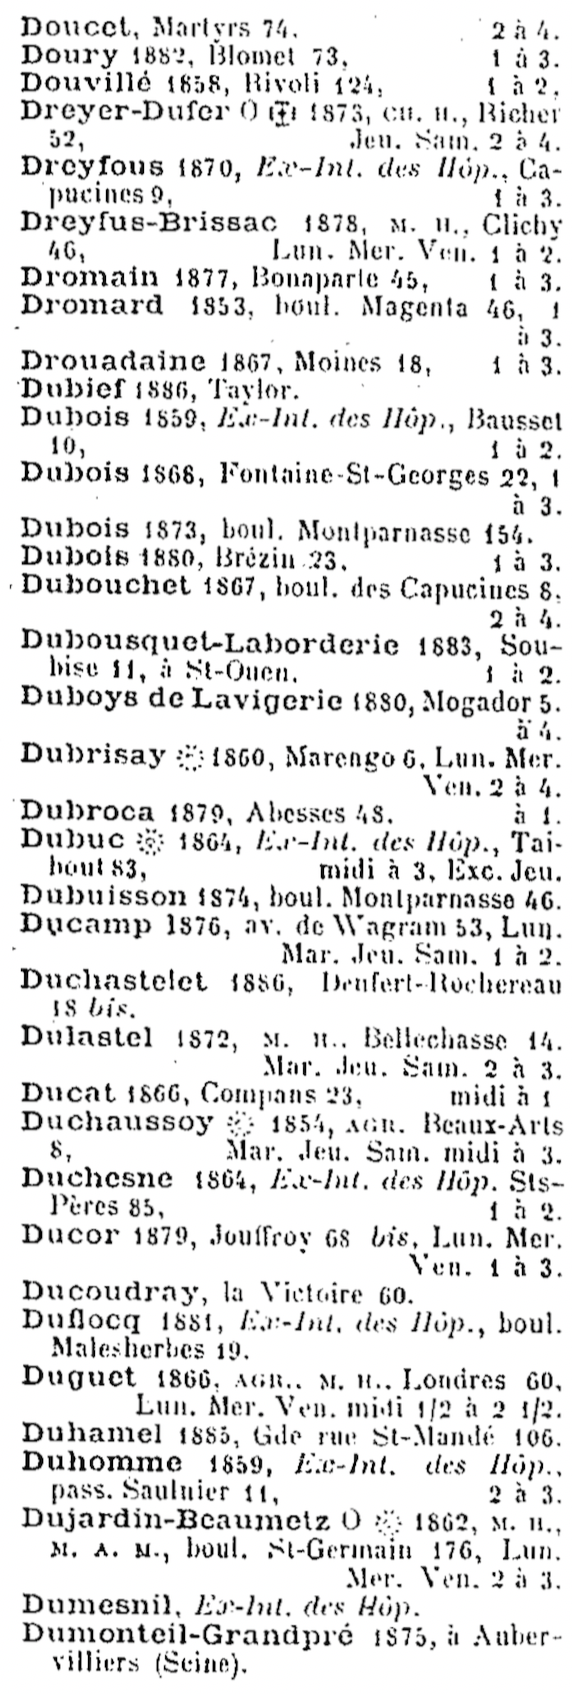
\includegraphics[width=0.49\linewidth]{Images/1887-0032-docteurs-en-medecine-et-en-chirurgie-paris-1.png}\hfill
    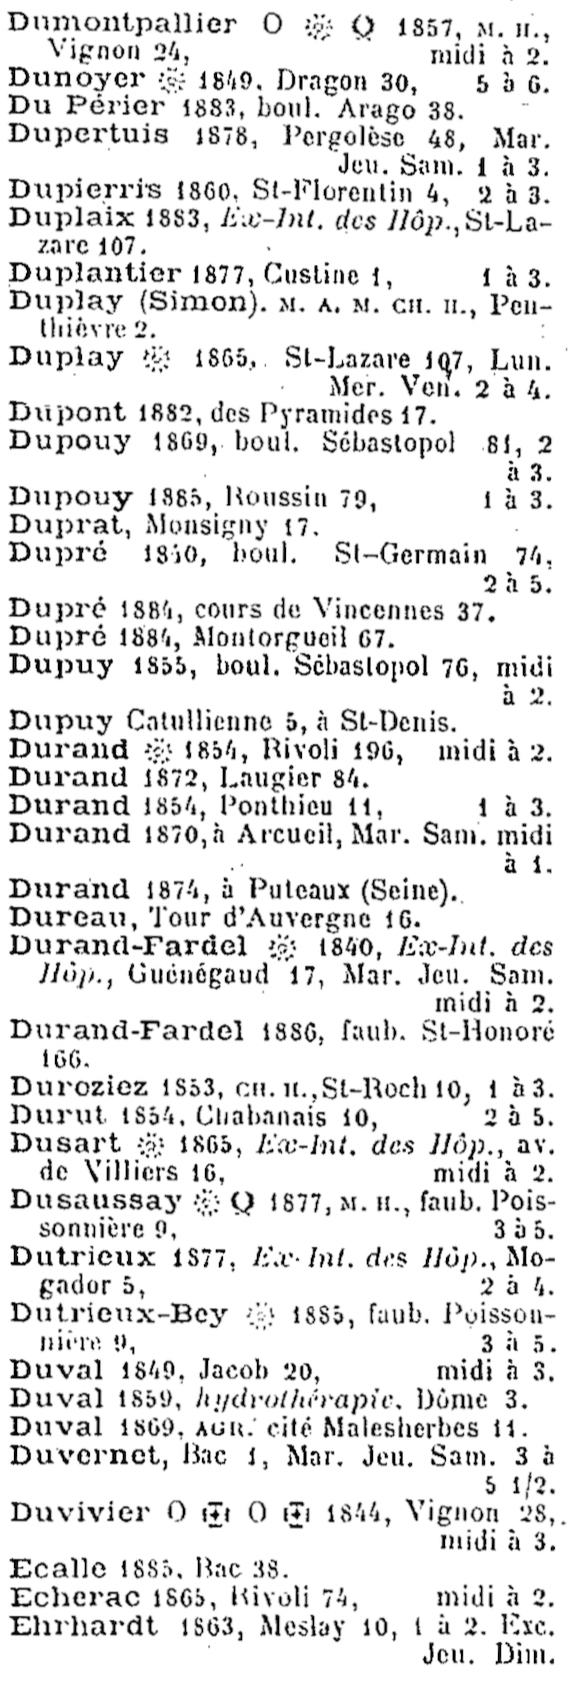
\includegraphics[width=0.49\linewidth]{Images/1887-0032-docteurs-en-medecine-et-en-chirurgie-paris-2.png}
    \caption{Doctors of medicine and surgery (Paris), Rosenwald Guide (1887, page 32): first (left) and second (right) columns.}
    \label{fig:1887-0032-paris-cols}
\end{figure}
\subsubsection{Model Configuration}
\label{sec:modle-config}
To satisfy the requirement of \textit{Orthogonal Independence} (Section~\ref{subsec:layer1}), we instantiate two distinct Systems using cross-company model pairs:
\begin{itemize}
    \item \textbf{System 1 ($S_1$):} $M_{1a}$ is \texttt{claude-sonnet-4-5} and $M_{1b}$ is \texttt{qwen3-vl-235b-a22b-thinking}. 
    \item \textbf{System 2 ($S_2$):} $M_{2a}$ is \texttt{llama4-maverick} and $M_{2b}$ is \texttt{grok-4-0709}. 
\end{itemize}
By design, each System uses heterogeneous models to reduce correlated failure modes (e.g., shared blind spots on degraded typography or consistent formatting hallucinations), thereby lowering the risk of \textit{Model Collapse} under agreement-based auto-labeling.

A stronger configuration would pair one MLLM with one traditional OCR engine, since classical OCR relies on fundamentally different recognition pipelines than end-to-end generative MLLMs and can therefore provide more complementary errors. In practice, however, our pilot experiments showed that the OCR outputs were too noisy for this setting: common failures included character-level misrecognitions and structural errors such as merging adjacent entries or mixing fields across different doctors. To keep the pipeline reliable and to reduce downstream human correction effort, we therefore use two MLLMs per System. In our data, MLLM outputs were consistently cleaner and more structured than the traditional OCR baseline, which substantially reduced the amount of manual correction required in the final verification step.



\subsection{Evaluation Metrics}
We employ a hierarchical metric strategy to proxy ground truth accuracy:

\begin{itemize}
    \item \textbf{Field Matching Rate ($P_{field}$):} A binary metric where $P_{field} = 1$ iff String($S_1$) $\equiv$ String($S_2$). This serves as the primary gatekeeper for the Golden Truth.
    \item \textbf{Character Matching Rate ($P_{char}$):} Calculated via normalized Levenshtein distance:
    \begin{equation}
        P_{char} = 1 - \frac{\text{Levenshtein}(L_a, L_b)}{\max(|L_a|, |L_b|)}
    \end{equation}
    This metric diagnoses the severity of disagreements (e.g., typo vs. hallucination).
    \item \textbf{Human Effort Reduction (HER):} Defined as the percentage of fields that bypass human review:
    \begin{equation}
        \text{HER} = \frac{N_{\text{total}} - N_{\text{reviewed}}}{N_{\text{total}}} \times 100\%
    \end{equation}
\end{itemize}


\subsection{Efficiency Test}
\subsection{Quality Test}


\subsection{Qualitative Error Analysis}
Disagreements at the First/Second Layer fell into three primary categories:

\subsection{Cost-Benefit Analysis}
How much time actually saved compared to double blind human annotation
% While the Double Triangle requires $4\times$ the inference compute of a single model, the primary cost driver in annotation is expert labor (historian time).
% \begin{itemize}
%     \item \textbf{Traditional Manual Annotation:} $\approx$ 120 seconds/entry.
%     \item \textbf{Double Triangle:} $\approx$ 5 seconds/entry (Expert review only on 2\% of data).
% \end{itemize}
% The framework delivered a \textbf{24x reduction in expert time}, effectively rendering the computational cost negligible in comparison to the labor savings.



\section{Limitation and Discussion}
\label{sec:limitation}


% The Double Triangle Annotation framework represents a paradigm shift in Human-in-the-Loop (HITL) workflows. By mathematically formalizing the relationship between Inter-Annotator Agreement and Accuracy ($P_o \approx \kappa \approx A$), we effectively invert the traditional annotation pyramid: machines handle the bulk of the cognitive load, while humans are elevated to the role of strategic conflict resolvers.
% For the specific task of digitizing 19th-century French Doctor Directories, this architecture delivered a Golden Truth benchmark with $>99.6\%$ precision at approximately $1/8^{th}$ the cost of traditional methods. Future work will explore the dynamic adjustment of the Layer 2 sampling rate based on real-time feedback from the Final Reviewer, potentially optimizing the efficiency-accuracy trade-off even further.
